\documentclass[conference]{IEEEtran}
\IEEEoverridecommandlockouts
% The preceding line is only needed to identify funding in the first footnote. If that is unneeded, please comment it out.
\usepackage{cite}
\usepackage{amsmath,amssymb,amsfonts}
\usepackage{algorithmic}
\usepackage{graphicx}
\usepackage{textcomp}
\usepackage{xcolor}
\def\BibTeX{{\rm B\kern-.05em{\sc i\kern-.025em b}\kern-.08em
    T\kern-.1667em\lower.7ex\hbox{E}\kern-.125emX}}
\begin{document}

\title{Controlling 3D Model of Human Hand Exploiting Synergistic Activation of 
The Upper Limb Muscles\\\
\thanks{
The Republic of Indonesia Government financially supported this study through Indonesia Endowment Fund for Education}
}

\author{\IEEEauthorblockN{Firman Isma Serdana}
\IEEEauthorblockA{\textit{Electronics Engineering Department} \\
\textit{Electronics Engineering Polytechnic Institute of Surabaya}\\
Surabaya, Indonesia \\
firmanisma@pens.ac.id}
}

\maketitle

\begin{abstract}
Surface electromyography (EMG) based control of hand exoskeleton has been developed in numerous methods, but a proportional control of multiple degrees of freedom (DOF) exoskeleton is still rarely seen in recent years. This paper proposes an alternative to the most recent solutions for proportionally estimating multiple DOFs of the hand. High-density electromyography (HD-EMG) was used to estimate the joint angle of five fingers in sophisticated gestures. The gestures were the ten alphabets of American Sign Language (A B C D F I K L O W). The association between HD-EMG and kinematics were mapped by using a neural network (NN) and k-Nearest Neighbour (kNN). The estimation accuracy was around 70-95 \% (R index) for the eleven DOFs in four normal-bodied subjects’ hand. Furthermore, kNN performed better than NN, even in the case of input feature reduction. The regression results also were able to distinguish 9 of 10 alphabets (except O), with the false interpretation was because of the identical muscle activity and kinematics between O and C. The approach described in this paper provides a practical solution to proportionally and simultaneously control multiple DOFs for hand exoskeleton.
\end{abstract}

\begin{IEEEkeywords}
High-density electromyography, hand kinematics, neural network, k-nearest 
neighbour
\end{IEEEkeywords}

\section{Introduction}
%Control of robotic hand based on electromyography (EMG) signal has been developed in numerous ways of methods and techniques. Starting from the simplest linear one which is only able to reproduce 2-3 degree of freedom (DOF) of hand movement (e.g. \cite{b1}), and more complex non-linear control, using the high order of DOF in the finger and wrist (e.g. \cite{b2} \& \cite{b3} respectively). Albeit abundant, the already commercialised control strategies are low in DOF (e.g. Ottobock Hands \cite{b4} and Openbionics \cite{b5}) and not particularly able to replicate human hand’s complex movement, especially in terms of digits control, hence its functionalities are quite limited.

%In the realm of complex hand movement estimation, most of the attempts use classification for its control (i.e. gestures are estimated discreetly not proportionally) \cite{b4}\cite{b5}. However, this method is not adequate to optimally utilise the more advanced robotic devices, for example, in continuous and sequential control \cite{b8}. A natural hand movement involves not only discreet movement, but also continuous, and simultaneous control of several DOFs. Some researchers have tried to estimate hand movement proportionally, although they focused more on the forearm and wrist movement \cite{b3}\cite{b9} limiting the finger movements as grasping/closing.

%The homunculus diagram \cite{b10} specifies 25\% of the neural area of the brain as hand and digit control, with each finger has their areas. This diagram is an indication of how important the use of hand movement in daily human life, either in object manipulations, or communications (e.g. sign language). Henceforth, excellent control of digit is quite essential to be replicated for practising complex gesture such as sign language.

The development of EMG based hand exoskeleton in recent years is mostly limited in grip/grasp gestures \cite{b11}\cite{b12}\cite{b13}, as the attempts to proportionally control multiple fingers through means of EMG are 
mostly meant for hand prosthetic. One research to estimate multiple fingers movement was performed by 
Smith \textit{et al.} at 2009 \cite{b14}. This study, however, did not incorporate the other more-distal joints of the finger;
it only estimated the metacarpophalangeal joints of the hand. At 2012, Hioki \textit{et al.} \cite{b15} proposed to estimate 
the proximal interphalangeal joints only because their range of motions are higher compared to other finger 
joints. This study used just four channels to estimate the angle, although compromises came from the 
multiple complex parameters the method needed for its configurations.

A further study to estimate multiple finger joints was performed by Ngeo \textit{et al.} \cite{b16}\cite{b17}. The study was 
able to predict all five fingers’ joints, including the more distal joints compared to previous studies (i.e. 
proximal and distal interphalangeal joints). The study however only estimated the joint angle from basic 
flexion-extension gestures (this is also true for other mentioned researches), it also incorporated a high 
computational regression model (Gaussian Process), which needed ten times more computational time 
compared to the neural network (albeit it required smaller training dataset). Previously Ngeo \textit{et al.} also 
controlled a finger exoskeleton to be compared with kinematics recording, although it was limited to index 
finger \cite{b18}.

%A recent study by Chen \textit{et al.} at 2019 \cite{b19} proposed the use of motor unit discharge to estimate five metacarpophalangeal joints of the hand. To decode the motor unit discharge, HD-EMG was used in the forearm. However, this study was still limited to the cross-correlation between the motor unit discharge and joint kinematics. The most recent study by Blana \textit{et al.} at 2019 \cite{b20} proposed the use of EMG driven biomechanical model to control a hand prosthesis proportionally. The biomechanical model gave a real-timeEMG driven proportional control of the hand. Although this study only estimated three DOFs of the hand (metacarpophalangeal joints of the thumb, index, and middle finger).

The study in this paper aims to present an alternative way of proportional hand control while also trying 
to enhance the results. High-density electromyography (HD-EMG), which was already proven to give an 
ample possibility of features in the previous study of proportional control of hand \cite{b9} and finger movement 
\cite{b2}\cite{b19}, was utilised in this study. We hypothesised that the high dimensionality of HD-EMG feature could maintain the control performance while only using less complicated regression methods such as Neural
Network (NN) and \textit{k}-Nearest Neighbour (kNN) (bigger dataset can enhance a less-complex model’s 
performance, especially in surface EMG case \cite{b21}). The high dimension features of HD-EMG recording 
were also analysed further to find the best optimal arrangement of surface EMG. In this case, and as previous 
studies always mentioned, to reduce the equipment’s complexity for future works involving EMG recording, 
we also deducted the dimension of the HD-EMG, by visual selection and principal component analysis 
(PCA).

%Contrary to the trending use of only extrinsic muscle for discreetly or proportionally controlling hand\cite{b16}\cite{b20} and following the use of intrinsic muscle in hand exoskeleton \cite{b11}\cite{b12}, we also added the intrinsic muscle to the control scheme. Following a previous study involving intrinsic muscle for hand control \cite{b22}, we hypothesised the addition of intrinsic muscle might improve the performance. We also investigated whether the use of only intrinsic muscle for the input of the control will be adequate for the proportional control of the hand. As opposed to the use of general bipolar surface EMG \cite{b23}, which limited the finger exoskeleton’s function to grip/grasp \cite{b12}, four-mm-spaced HD-EMG was utilised to give a spatially more evident feature of the small intrinsic muscle activities.

%Unlike Celadon \textit{et al.} \cite{b2} and Barsotti \textit{et al.} \cite{b24} (which also used HD-EMG), we estimated the kinematics of the fingers rather than their forces. The kinematics of the finger were concurrently recorded with the HD-EMG recording. This kinematics recording, as in Ngeo \textit{et al.} study \cite{b16}, was used for the training and testing target of the proportional control. In contrast to Ngeo \textit{et al.} \cite{b16}, the gestures recorded were not basic flexion/extension, but sophisticated gestures in the form of a selection of American Sign Language (ASL) alphabets. The complex gesture was considered to pursue the dexterity of real human fingers in proportional control of hand exoskeleton.

%To summarise, this study provides a new proportional control method to estimate complex gesture of finger movement. This new method incorporates the multiple DOFs of human fingers to be simultaneously estimated by HD-EMG signals. Neural Network and \textit{k}-Nearest Neighbour are utilised to map the HD-EMG feature with the kinematics recording.


\section{Methods}

\subsection{Subject}
Following the previous development of novel proportional control of the hand \cite{b9}\cite{b16}, healthy 
abled/normally-limbed subjects were considered. Four male subjects (aged 24±2.58) volunteered in the 
study. All of them were dominantly right-handed. Before the experiment, all the subject signed informed 
consent following the ethics of the research. Ethics approval was given for the experiment.
\begin{figure}[htbp]
\centerline{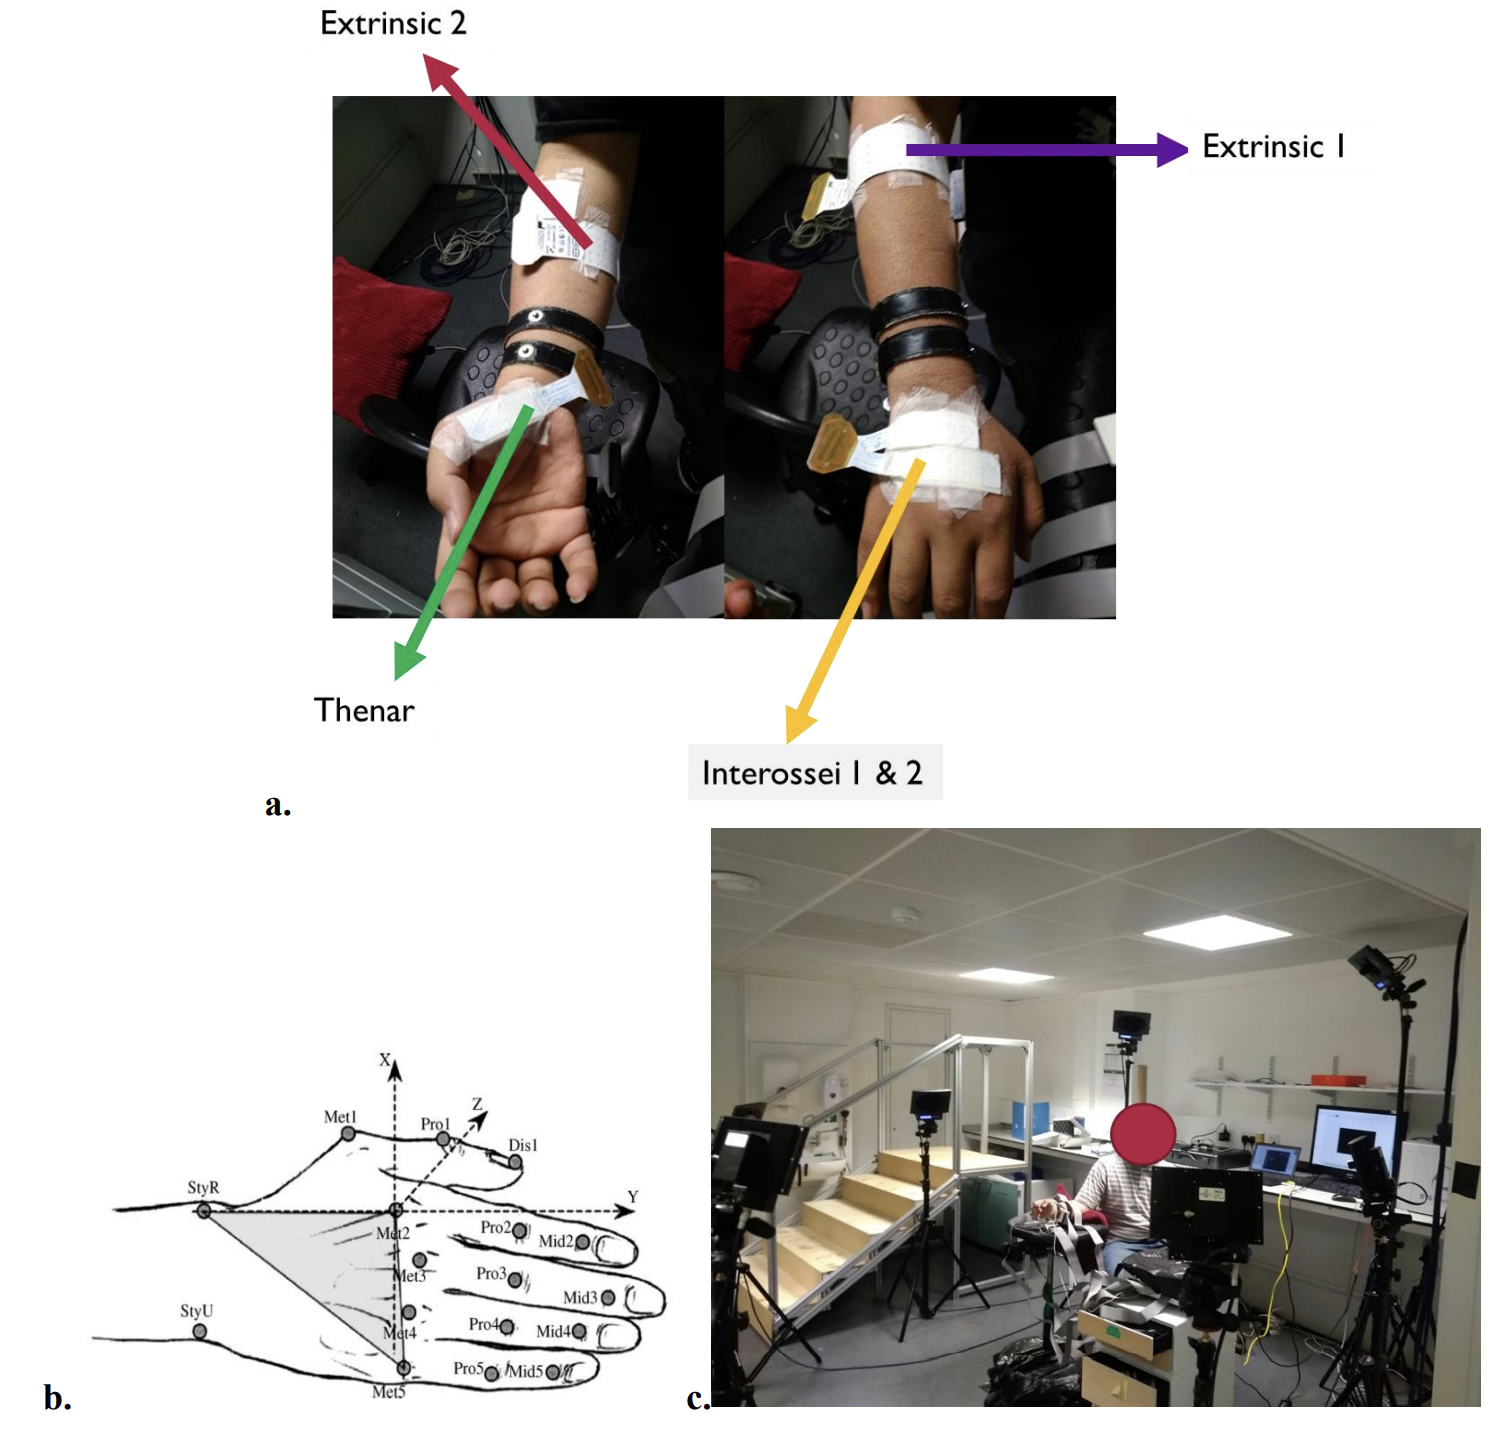
\includegraphics[width=\columnwidth]{figure1.png}}
\caption{\textbf{a.)} Placement of the HD-EMG grid, two 8 mm grids on the forearm (Extrinsic 1-2), and three 4 mm grids on the hand (Thenar, Interossei 1-2). \textbf{b.)} Marker placement for kinematics recording \cite{b25}, StyR-U: the styloid process of ulnar and radius respectively, Met1-5: metacarpal, Pro1-5: proximal phalanges, Dist1: a distal phalanx of the thumb, and Mid2-5: middle phalanges of other fingers. \textbf{c.)} The position of the subject, surrounded by eight motion capture cameras focusing on the hand of the subject}
\label{figure1}
\end{figure}

\subsection{Data Acqusition: HD-EMG}
The grids were placed on the right arm muscle responsible for the flexion and extension of the fingers (i.e. extrinsic and intrinsic muscle of the hand). Two types of HD-EMG were used; 8 mm (GR08MM1305) and 4 mm (GR04MM1305) spaced 64 channels grids. Each of the grid has 13 columns and five rows (OT Bioelettronica, Torino, Italy). Two 8-mm-spaced grids were placed around the circumference of the forearm (positioned on the most muscular part of the forearm) to record the activity of extrinsic muscle of finger (e.g. extensor and flexor digitorum muscles) following Muceli and Farina suggestion \cite{b9}. The 4-mm-spaced grids, three in total, were placed on the intrinsic muscle of the hand. Two of which were across the dorsal side of the hand (interossei muscles), placed in adjacent to each other to cover the whole dorsal side. Another one was placed on the palmar side of the thumb (thenar eminence muscles) \textbf{(Figure 1a)}. Before placing the HD-EMG grids, the subject’s skin was necessarily shaved for reducing noises from the hair and lightly cleaned 
with alcohol.

Monopolar HD-EMG signals were recorded with 150 gain, sampled with a frequency of 2048 Hz, cut-off with a bandpass filter of 10-500 Hz frequency, and digitally converted with 16 bits precision 
(Quattrocento, OT Bioelettronica, Torino, Italy). Two ground electrodes placed on the wrist of the right arm were used for the references.

\subsection{Data Acqusition: Kinematics Recording}
Seventeen small 8 mm infrared reflective markers (semi hemisphere) were placed on the bony marks 
at the dorsal side of the hand \textbf{(Figure 1b)}. Starting from distal side of the hand, 2 markers were placed on 
the styloid process of radius and ulnar bone (StyU-R), 5 markers on the head of the metacarpal and proximal 
for each finger (Met1-5), 4 others were placed on heads of middle phalanges (index-little finger) (Pro2-5), 
and the last one on the head of distal phalange of the thumb (Dis1) \cite{b25}. There were no markers at the distal 
head of index-little fingers because the calculation of distal interphalangeal joints was not considered.

These markers were captured by using a motion capture system consisted of 8 infrared cameras (Smart-DX 6000, BTS Bioengineering, Quincy-USA) and were analysed by using motion analysis software
(SmartTracker application, BTS Bioengineering, Quincy-USA). After considerations, the camera placement 
setup was: 6 cameras were located at the front with the same height as the subject, and two other cameras 
were fixed at a higher position behind the subject \textbf{(Figure 1c)}. The positioning of cameras helped to reduce 
the loss of the marker (a common problem with motion capture system) as this configuration helped 
pertaining 2-3 cameras to capture all the markers.

The kinematics recording sampling rate was adjusted to 250 Hz. Then, the calibration volume was set 
to extra small (20 cm in all axis) in conjunction with the extra-small markers (8 mm), to make sure a clear 
capture of the hand kinematics. This configuration was also used to avoid the flickering and noise of motion 
capture caused by the markers switching and closely spaced markers errors

\begin{figure}[htbp]
\centerline{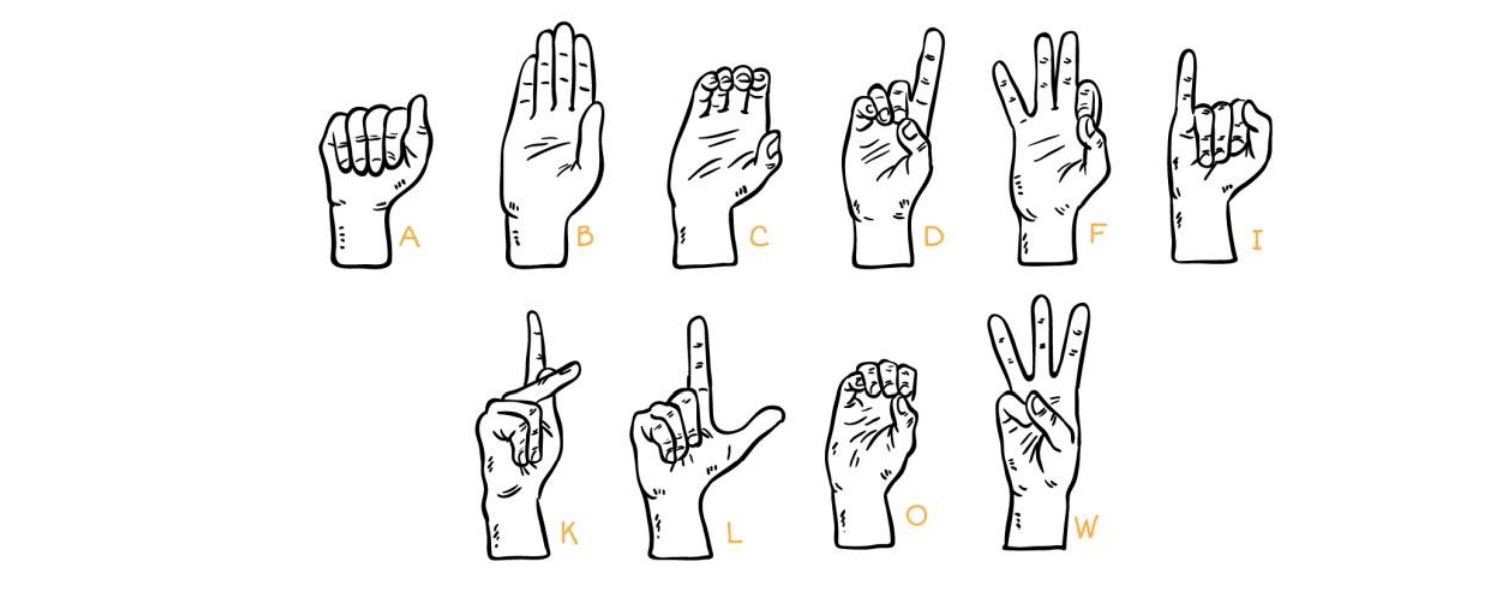
\includegraphics[width=\columnwidth]{figure2.png}}
\caption{10 alphabets of American Sign Language used for the experiments \cite{b26}.}
\label{figure2}
\end{figure}

\subsection{Experimental Procedures}
%The subjects were seated in a standard chair and asked to position their elbow in the small table. This positioning can be managed to the subject desires (the height, the rotation of the chair and table) to guarantee the comfortability aspect of the procedure. While in this position, the subjects were asked to maintain a static position in the recorded hand avoiding any movement except finger movement, this was to get a clear recording of finger muscle EMG and avoiding muscle activity responsible for the wrist motions. The distal side of the hand was required to face toward the front cameras, while the dorsal and palmar sides werelooking at the side cameras. The hand of the subject should not supinate, pronate or radial-ulnar deviate while recording (although in resting state). This was not only for avoiding other muscle to be activated but also ensuring all markers always to be captured by cameras.

American Sign Language (ASL) gestures were mostly used for classification-based EMG hand control 
\cite{b27}, but in this study, the gestures were proportionally tracked and recognised. The subjects were tasked to 
perform ten alphabets gestures \textbf{(Figure 2)} from a resting position. Of all alphabets and numeric ASL gesture, 
these ten were chosen according to their variability \cite{b28} (Section 3.A.), and their feasibility for motion 
capture (the finger will not block the markers). Before the experiment, the subjects were trained to avoid 
gesture lag while in the experiment. In the task, the subjects were given two auditory cues to start and stop 
the gestures (about 4 seconds in between). The resting position, which was also recorded 1 second before 
and after the gesture, was when the subject did not exert force on finger muscles. Between the two cues, the 
subjects were asked to maintain the gesture normally for about 4 seconds, while avoiding any exertion of 
excessive and non-finger forces. The ten alphabets were repeated three times in random order; totalling of 
30 data were recorded from each subject. In between recording, the subjects might take a rest at their 
discretion, but after 15 recordings, the subjects were asked to rest their hand for avoiding fatigue.
Both the data (HD-EMG and kinematics) were concurrently recorded from the subjects’ right arm. 
Mirrored movements \cite{b9} were not considered because of the complexity of ASL gestures might hinder the 
recorded data and prolongs the subject’s training of the gestures. A rectangular signal, generated by an 
Arduino Uno, was used to synchronise two different systems (Quattrocento and Smart DX 6000). This 
synchronisation signal was triggered by the operator at the same time with the start auditory cue and ceased 
in synchrony with the stop auditory cue to truncate the data and ignore any undesired recordings.

\subsection{Data Post Processing: HD-EMG}
An offline bandpass filter (4th order zero-lag Butterworth digital filter with a cut-off frequency of 20-
400 Hz) was applied to the HD-EMG signals. This was to filter out undesired noises such as motion artefacts. 
After that, the EMG recordings were visually checked to remove the bad-contact channels (the amount of 
the bad channels varied on each subject). Then, the monopolar recordings were transformed into bipolar 
channels along to the vector of muscle fibre (reducing the 320 channels to 267) to ensure a common-mode 
rejection rate was applied to the recordings \cite{b9}. The Fourier analysis for the post-processing showed the HD-EMG data had an optimum frequency of less than 30 Hz. To only acquire the muscle activity, a 
16 Hz low pass filter (2nd order, zero lag, Butterworth digital filter) was also applied to the HD-EMG data 
\cite{b9}\cite{b29}.

From here, non-overlapping root means square (RMS) feature of the HD-EMG signals were extracted 
with ~15 milliseconds window steps, resulting in low control rate of ~60 Hz. The use of RMS is mostly 
applied in EMG feature extraction because it has a reasonable estimation of EMG activity over a time 
window \cite{b2}\cite{b30}. Contrary to Muceli and Farina \cite{b9} and Ngeo \textit{et al.} \cite{b16}, the HD-EMG signals (and its 
derivate feature) were not down-sampled to similar rate with the kinematics recording to avoid information 
loss.

\begin{figure*}[htbp]
\centerline{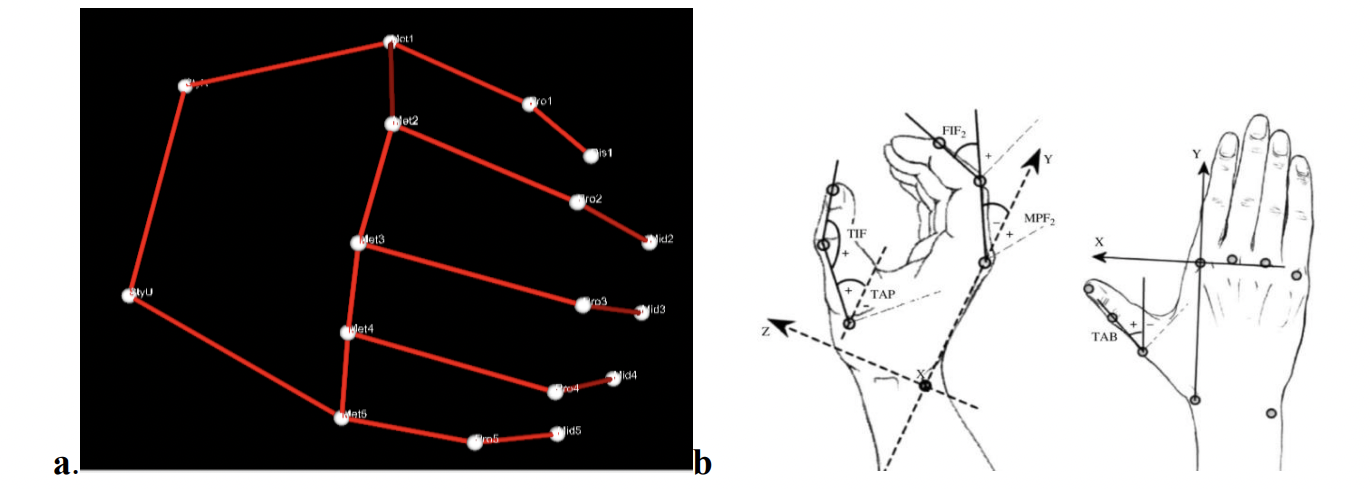
\includegraphics[width=\textwidth]{figure3.png}}
\caption{ \textbf{a.)} The model of the hand following \textbf{Figure 1b} with some links that interconnected each of 
the markers. This model can be the base for designing the soft exoskeleton. \textbf{b.)} Joint angle calculation 
based on Carpinella \textit{et al.} \cite{b25}, FIF = proximal interphalangeal joint flexion angle; MPF = 
metacarpophalangeal joint flexion angle; TIF = thumb interphalangeal joint flexion angle; TAP = 
thumb ante position angle; TAB = thumb abduction angle.}
\label{figure3}
\end{figure*}

\subsection{Data Post Processing: Kinematics Recording}
At first, the kinematics recording produced the position of the markers in 2D space for each of the 
motion capture camera. Then using Smart Tracker software (BTS Bioengineering, Quincy-USA), the 2D 
recording was reconstructed into 3D space. A linked model was applied to the markers to give a visual cue 
of a real hand model (\textbf{Figure 3a.}). Eleven 1-dimensional angles were then calculated (\textbf{Figure 3b.}) using 
Smart Analyzer software (BTS Bioengineering, Quincy-USA). The calculated angle with their respective 
marker reference can be seen in \textbf{Table 1}. The distal interphalangeal joints of the index-little finger were not 
measured because of its low impact in hand gestures \cite{b31}, and its near-identical movement with the proximal 
interphalangeal joints (anatomically both joints have common flexor and extensor) \cite{b16}. Similar to distal 
interphalangeal joints, the abduction angles of index-little fingers were also omitted from the calculation.

The joints angle data was then up-sampled to have a common sampling rate with the HD-EMG data 
(2048 Hz). As mentioned in section 2.C, some markers might be lost in the kinematics recording process. 
Hence an interpolation (or extrapolation if markers loss happens at the start/end of the recording) was performed. The noisy kinematics data (happened because of the vibrating markers) was also smoothed using 
moving average Gaussian filter (equal to a low-pass filter with a cut off frequency of 1 Hz). This filter was 
chosen because its output resembled a natural hand movement compared to the other techniques.

\begin{table}[]
    \centering
     \caption{ The joint and their own three markers used to calculate their angles. 2-5 specify the finger from 
the radial side (index, middle, ring and little finger)
    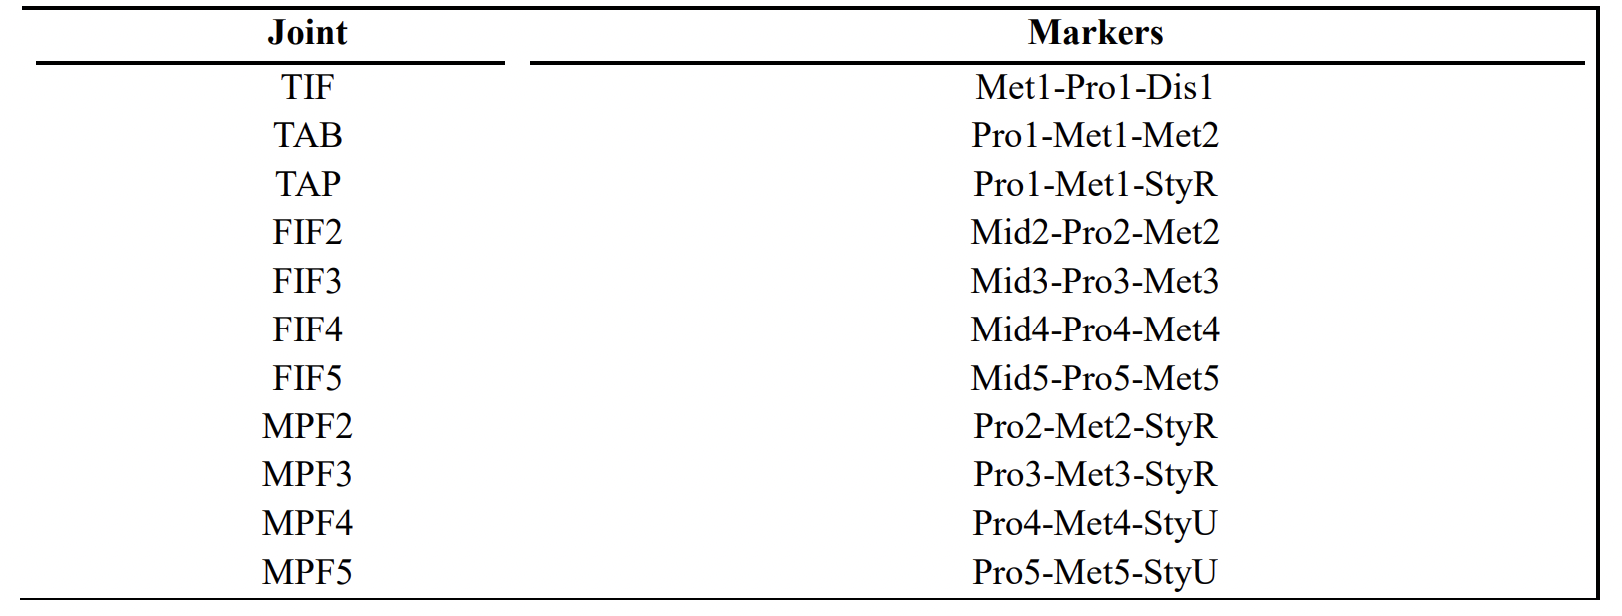
\includegraphics[width=\columnwidth]{table1.png}
}
    \label{tab}
\end{table}

%\subsection{Feature Analysis}
%The high dimension of HD-EMG gives an excellent possibility of features as its small spaced channels have a better chance to capture most of the muscle activity \cite{b23}. However, this also means that the adjacent channels are highly correlated with each other (the dataset has redundancy). 
%The redundant information of HD-EMG can be reduced by visual selection and its principal components. In this study, the visual selection was based on the vector of the muscle (i.e. for Extrinsic 1-2, Interossei 1-2 it was selected horizontally, but for Thenar, it was vertically) \cite{b9}. Horizontal Linear arrays of the bipolar channel (14) and seven equally spaced channels were selected from Extrinsic 1-2 and Interossei 1-2 grids. In the Thenar grid, it was selected vertically. Hence, five vertical linear arrays and three equally spaced channels were selected.

%A principal component analysis on the RMS features was done for each of the grids \cite{b9}. The first principal components (PC) sufficed to explain ~70 \% of the RMS features’ variance in all subjects.Therefore, we investigated if 14-7-1 first components could suffice for the input for training the regression model (see section 3.A for detail).

%As previously explained in section 1, we also investigated whether the use of each hand muscle type (extrinsic and intrinsic muscle) might result differently. Here the features were also divided into two groups depending on their recorded muscle. The Extrinsic 1-2 grids were grouped as an extrinsic feature, where the Interossei 1-2 and Thenar grids were grouped as an intrinsic feature.

%Then, all the feature configurations were used in the training and testing of the regression. Their performances were compared to each other. Separate 3-way Analysis of Variance (ANOVAs) with three main factors (subject, regression method, and input features) was used for each of the angles. A further posthoc Tukey-Krame’s test was also used to check the significant difference for each factor’s groups if there is any significant main factors and interactions in 3-way ANOVA. To know the specific difference without considering other factors, a focused ANOVA was also performed between specific factors.

%An investigation about the output features was also conducted to know whether it is possible to reduce the redundant 11 DOFs of the hand model \cite{b28}\cite{b32}. The result of the analysis was not implemented becausethe focus of this study was only to estimate multiple DOFs of the hand simultaneously. However, it could be used as a method to recognise the ASL gesture.

\subsection{Joint Angle Estimation}
Although the EMG activity is highly correlated to the muscle’s force \cite{b2}\cite{b24}, some studies found that 
it can also be applied to estimate the angle of the joints \cite{b9}\cite{b16}. In this study, NN and kNN were used to train 
the regression model between the HD-EMG and joint angle data.

The NN used was a convolutional NN with two hidden Rectified Linear Unit (ReLU) layers. The
convolutional NN was considered following its excellent performance in complex bio-signal prediction while still having low computational demand \cite{b33}\cite{b34}. The NN’s two hidden layers had 100 and 50 neurons,
respectively (chosen as the best overall hyperparameters). The input layer’s neurons depended on the number 
of input feature used, and the output layer has one single output, meaning there were eleven separates
different NNs were trained for each angle (estimating all angle with single NN gave a mediocre
performance). However, for fair comparisons, the hyperparameters of the NNs were not uniquely modified 
for each of the angles. The dataset was three-fold divided for cross-validation while training the NN, where 
2 out of 3 were used as training/validation dataset (70/30 \% respectively) and the last one used as an unseen 
dataset for testing the NN performance.

Although heavily used for classification problems, \textit{k}-Nearest Neighbour (kNN) can also be used for 
regression or estimation, primarily if used for estimating a single value with a rich dataset as input \cite{b35}. 
Therefore, this simple model was also used with the same input and output characteristic as NN in the 
previous explanation. The k hyperparameter was set to 5 (best overall) for each angle estimation for fair 
comparisons.

The output of the regression was post-processed further to resemble natural movement, using the same 
process with the post-processing of kinematics recording (section 2.F). It was smoothed with Gaussian 
method and then low pass filtered (2\textsuperscript{nd} order, zero lag, Butterworth digital filter, cut-off frequency 7 Hz) 
\cite{b9}\cite{b16}.
For assessing the accuracy of each joint angle estimation, two performance metrics were used in this 
study. The first metric was Pearson’s Correlation Coefficient (R), and the second was the root mean square 
error (RMSE) between the prediction output and measured joint angles \cite{b16}. The R-value indicates the 
variability between predicted and actual values, while the RMSE indicates the residual error between those 
values.

\section{Results}
\begin{figure}
    \centering
    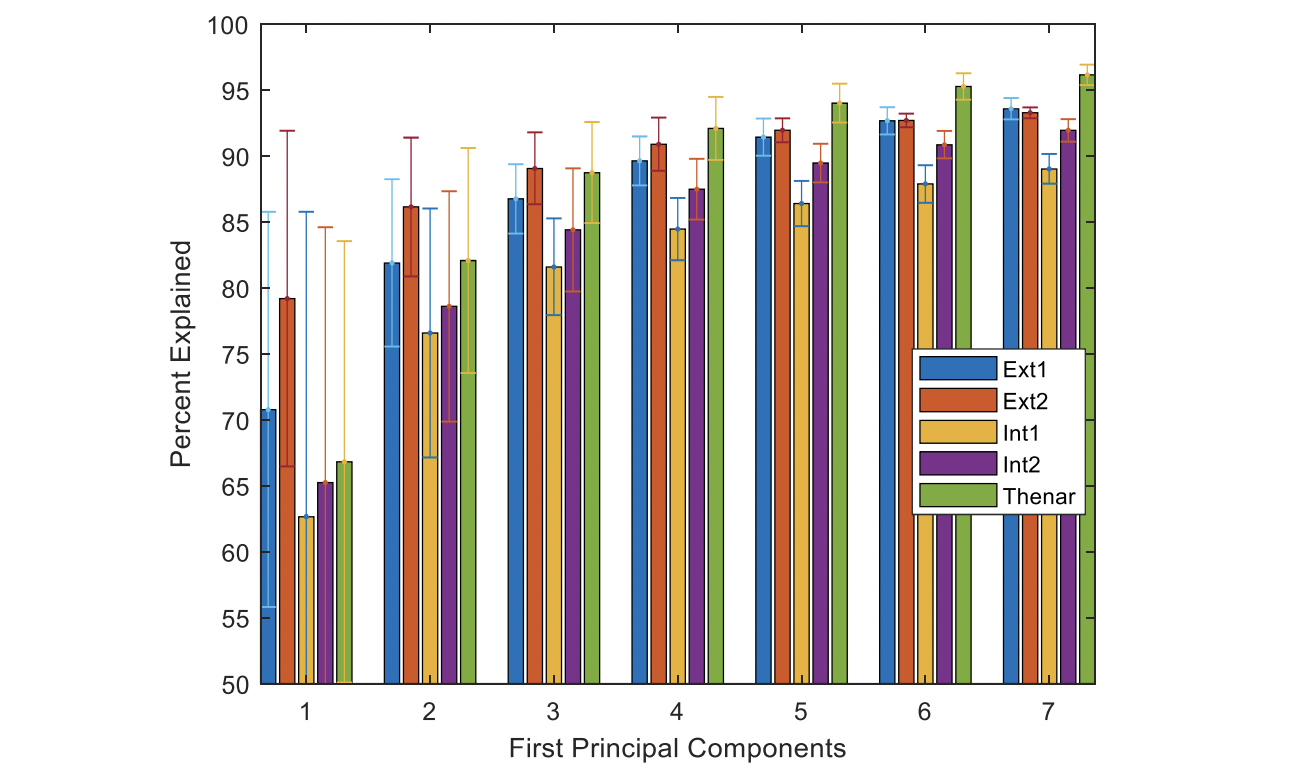
\includegraphics[width=\columnwidth]{figure4.png}
    \caption{The percentage of explained variance in each of the grids for seven first principal 
components. The Ext1-2 are Extrinsic grids, Int1-2 are Interossei grids, and Thenar is the thumb grid.}
    \label{figure4}
\end{figure}

\subsection{Data Analysis}
The high dimension of HD-EMG’s gave redundant information because of its high number of 
electrodes/channels. In the development phase, this will be useful for finding the best optimum EMG
configuration for future implementation. Therefore, in this study, PCA of HD-EMG grids was used to 
analyse the possible optimum EMG configuration. The first PC overall already explained ~70\% of the data 
(70.78 ± 14.98 for Ext1, 79.18 ± 12.72 for Ext2, 62.67 ± 23.098 for Int1, 65.24 ± 19.36 for Int2, and 66.81 
± 16.73 for Thenar) (\textbf{Figure 4}). The first 7 PCs, however, already explained ~90\% for each grid which 
constituted for the standard of a good explanation of entire data \cite{b9}\cite{b23}. Therefore, in this study, the 7 and 1 
PC of the dataset was used for training the regression model. For a closer perfect explanation of entire data, 
14 first PCs was also used (explained $>$95 \%).
A repeatability test (Analysis of Variance) of finger angles showed the kinematics recording are all 
repeatable (\textit{p}$<$0.05) for each Alphabets in all four subjects (Carpinella \textit{et al.} 2006 \cite{b25}). However, 
individually, each subject had several p-values over 0.05, although it varied and did not commonly happen 
in certain angles or alphabet.
The high DOFs of the hand, according to Santello \textit{et al.} \cite{b32} and Weiss and Flanders \cite{b28}, may also be 
reduced further to several DOFs. 4 PCs of the kinematics data already explained $>$90\% of the data (\textbf{Figure 5a.}). Although, in this study, the dimension of kinematic data was not reduced in the regression phase as the 
study only focused on simultaneous control of multiple DOFs of the hand. However, it is still possible to
design proportional control by reducing the kinematics dimension \cite{b36}.
Using the PCA could give information about the variability of the kinematics dataset. The PCs of the
alphabets have distinct variability for each other in all the subjects. The distribution of 2 first PCs in Figure 
5b explained that the alphabets used did not overlap with each other, not even their standard deviation. The 
closest alphabets were only D-K and O-C (because they are identical, see \textbf{Figure 2}).

\begin{figure}
    \centering
    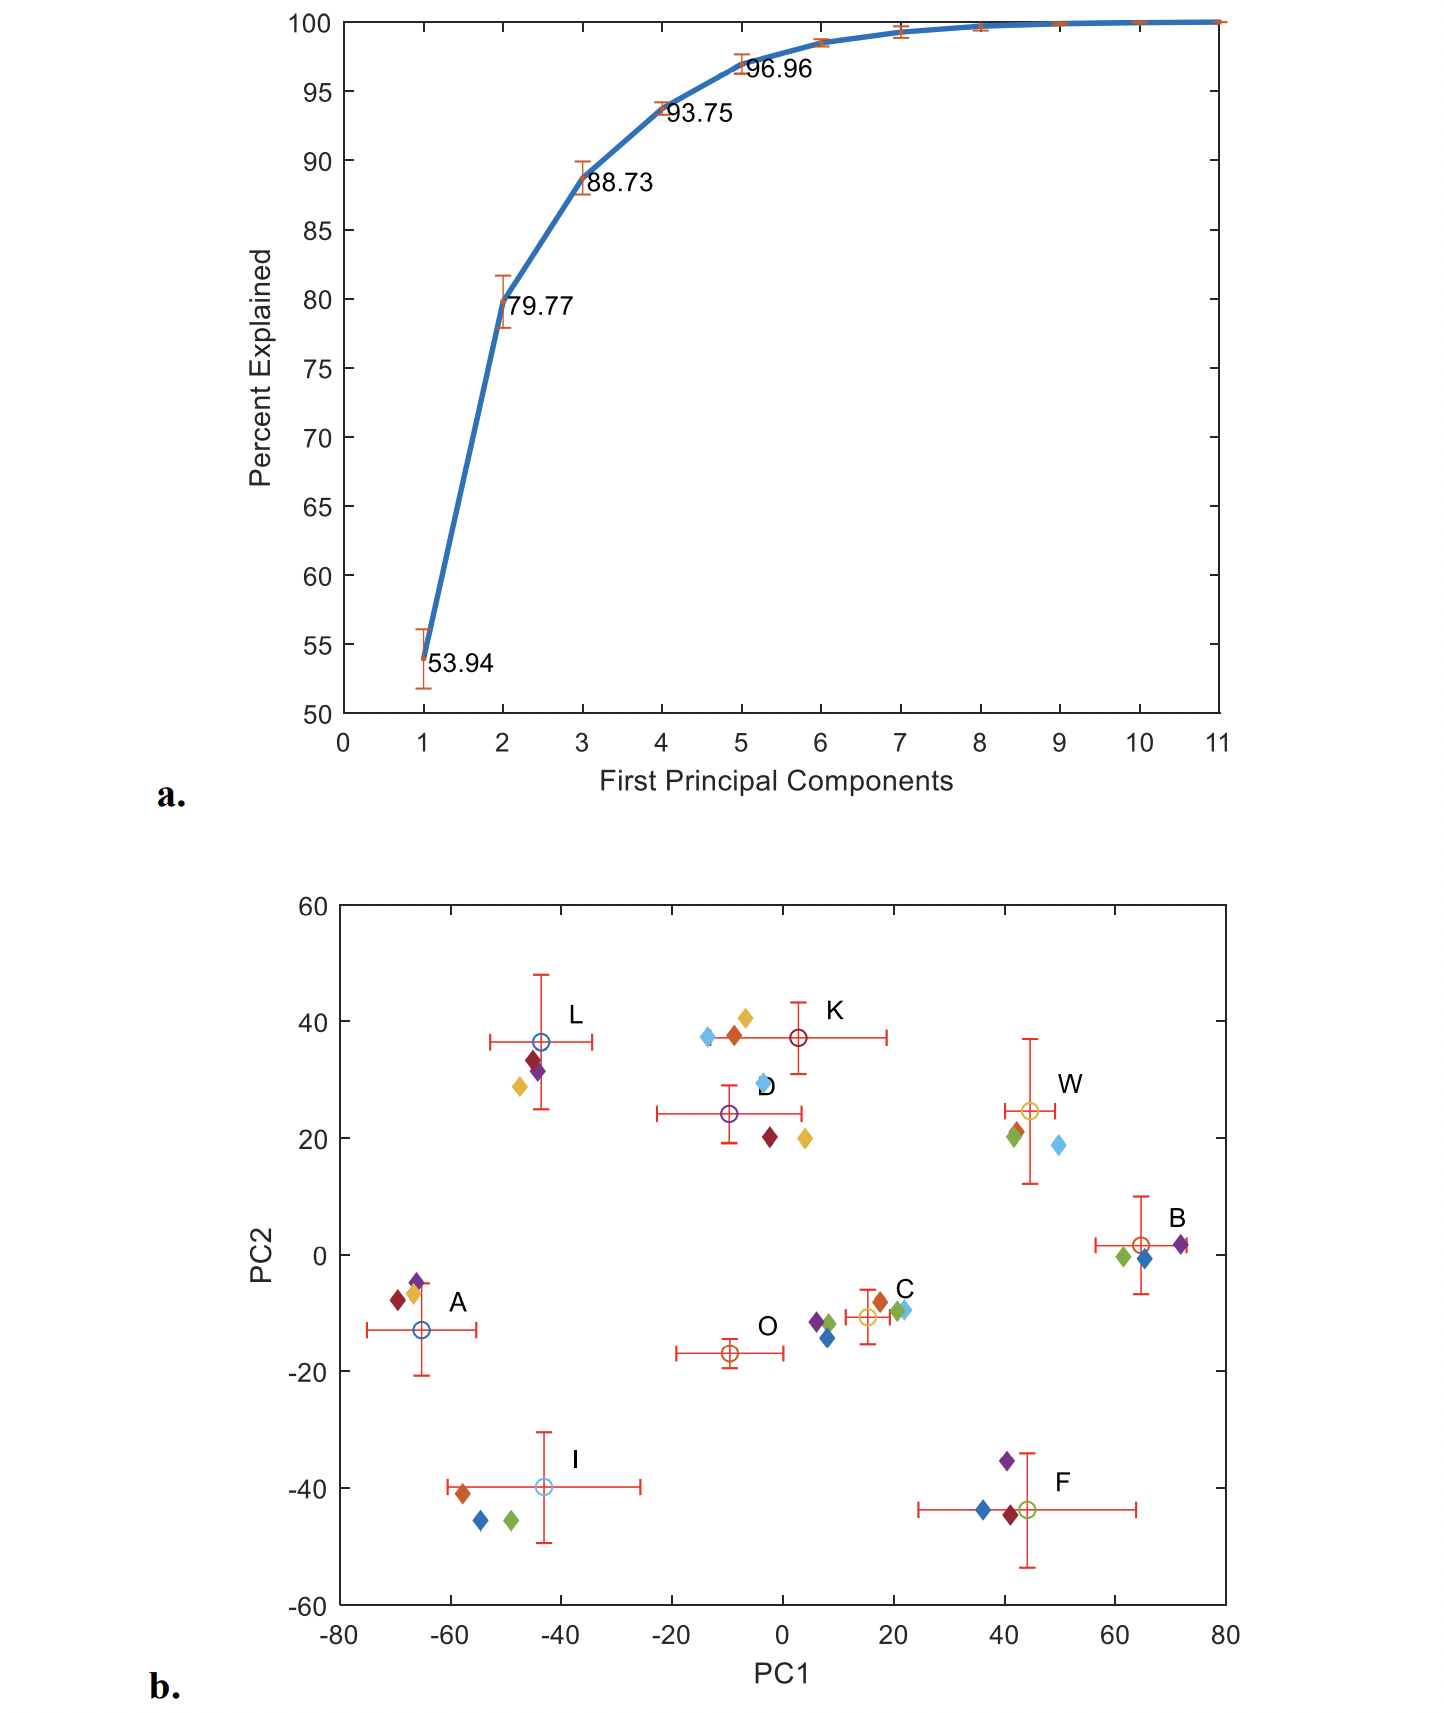
\includegraphics[width=\columnwidth]{figure5.png}
    \caption{\textbf{a.)} Percentage of kinematics data explained by its PCs. 2 PCs already explained ~80 \% of 
the data, although in \cite{b28}, using all ASL alphabets, 4 PCs were needed to explain $>$80\% of the data. 
\textbf{b.)} The scatter plot for the average of 2 first PCs in kinematics dataset of all subjects. Each unfilled 
dot represents the ASL alphabets used in the experiment, along with their standard deviations. The 
diamond-shaped markers were the two first PCs of the predicted joint angles in Subject 3 using kNN 
with average RMSE = 10.78 ± 4.64 \% and R = 80.65 ± 6.92 \% in all DOFs.}
    \label{figure5}
\end{figure}

\subsection{Overall Result}
\begin{figure}
    \centering
    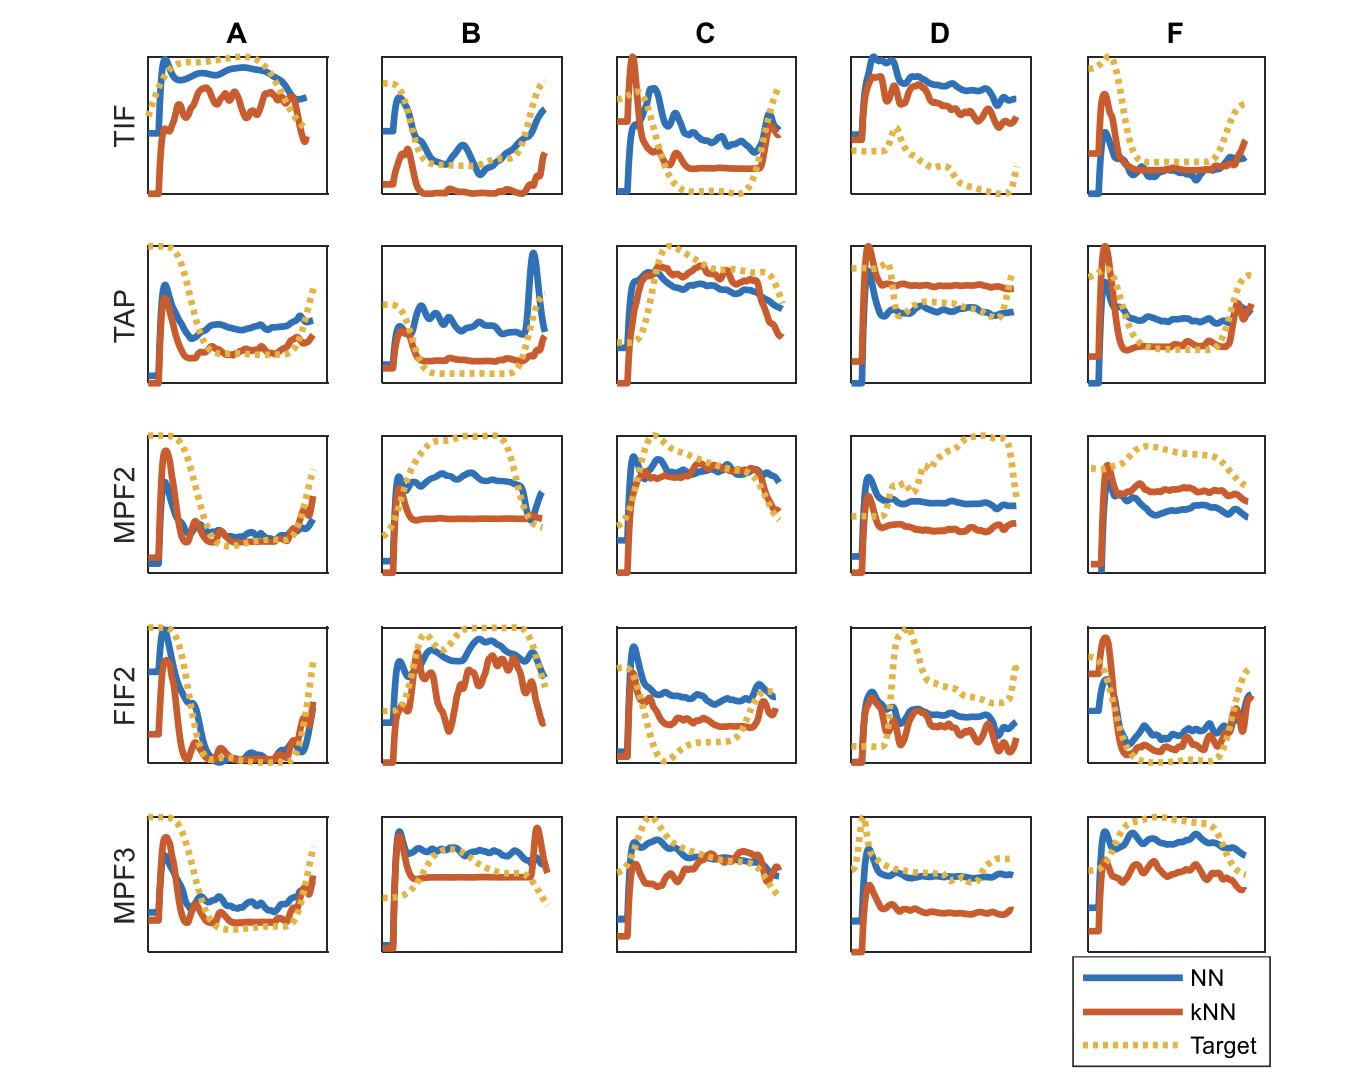
\includegraphics[width=\columnwidth]{figure6.png}
    \caption{An example of joint angle estimation between Neural Network (NN), k-Nearest Neighbour 
(kNN) and its actual output. Only A B C D F gestures, TIF, TAP, MPF2, FIF2 and MPF3 joint angles 
were shown for clarity. The dataset used was from Subject 3 
using all bipolar channels as input. The overall performance for NN was R = 72.67 +/- 4.55 \%, RMSE 
= 10.08 +/- 0.25 \%; and for kNN was R = 80.4 +/- 0.82 \%, RMSE = 11.37 +/- 0.83 \%.}
    \label{figure6}
\end{figure}

After the regressors were trained, all eleven joint angles were simultaneously estimated. \textbf{Figure 6}
represents the joint angle estimation result using NN and kNN. Both the regressors were trained with 66 \% 
of the dataset then performed against the remaining third of the dataset. Overall, both the regressors, in this 
case, followed the target closely, although in some joint angles and alphabets it deviated significantly. In some good cases, however, the R-value could go as high as ~95\% in 
metacarpophalangeal joints (MPF and TAP), and in proximal interphalangeal joints (FIF and TIF), as high 
as 90 \%. The abduction of the thumb (TAB), however, performed poorly compared to other joints. In RMSE 
terms, overall the residual error was about 10 \%, with the lowest possible RMSE could go as low as ~5\%.

For comparing each of the parameter modified in the regression process, \textbf{Figure 7} can be used. The 
RMSE metric was not giving a clear significant difference, between different input feature configurations, 
although the estimation accuracy was clearer in R. The best configuration was using full grids as the input 
feature (as also reported by Muceli and Farina \cite{b9}) with kNN as the regression method (Overall R= 78.09 ± 
5.49 \% and RMSE= 12.21 ± 5.09 \%). Using PCA1 in NN gave the most inferior performance, albeit faster 
(Overall R= 65.03 ± 2.66 \% and RMSE= 11.67 ± 4.64 \%). Ordering the performance, although not 
significantly different in most angles, PCA14 performed better than PCA7 and Sel14 performed better than 
Sel7.

In NN and kNN regressor, significant differences were not found between PCA14 and Sel14 input 
features configuration (R and RMSE wise, except in TAB angle). Between PCA7 and Sel7 at NN, however, 
significant differences were found in some of the angles (MPF2, MPF3, MPF4, \textit{p}$<$0.05 R-value only). In 
NN, a full grids feature displayed significantly different result compared to both reduced features in most 
angles (using PCA and selection, \textit{p}$<$0.01 at most angles). NN and kNN did not have any significant 
difference when using full grids as their input features. Although using all factor (including feature 
dimension factors), posthoc Tukey-Krame’s test revealed that surprisingly kNN, overall, performed better 
than NN regardless of the feature dimension (about 4 \% better, \textit{p}$<$$<$0.001).

The use of extrinsic only grids, overall, performed poorly compared with the full grids and even 
intrinsic grids only (R=~60\% and RMSE=~20\%). Some significant differences between extrinsic only and 
full grids configuration were also found in most angles with \textit{p}$<$0.05. Interestingly, the intrinsic grids feature 
had no significant difference in most angle compared with full grids feature (R$>$~70\% and RMSE$<$~11 \%). 
By using two first PCs of the kinematics recording and prediction, the regression results could be 
classified into its gestures (not fully explored in this paper). As seen in \textbf{Figure 5b}, most distinct alphabet 
predictions (9 of 10 ASL gestures) gave a more unambiguous classification as they fell into the areas of real 
alphabets measurement (or closer to the real alphabet). However, the prediction result of identical alphabets 
(O-C) could be falsely interpreted. The O predictions were only in the areas of actual C, giving it a possible 
false-positive result of O prediction as C.

\begin{figure}
    \centering
    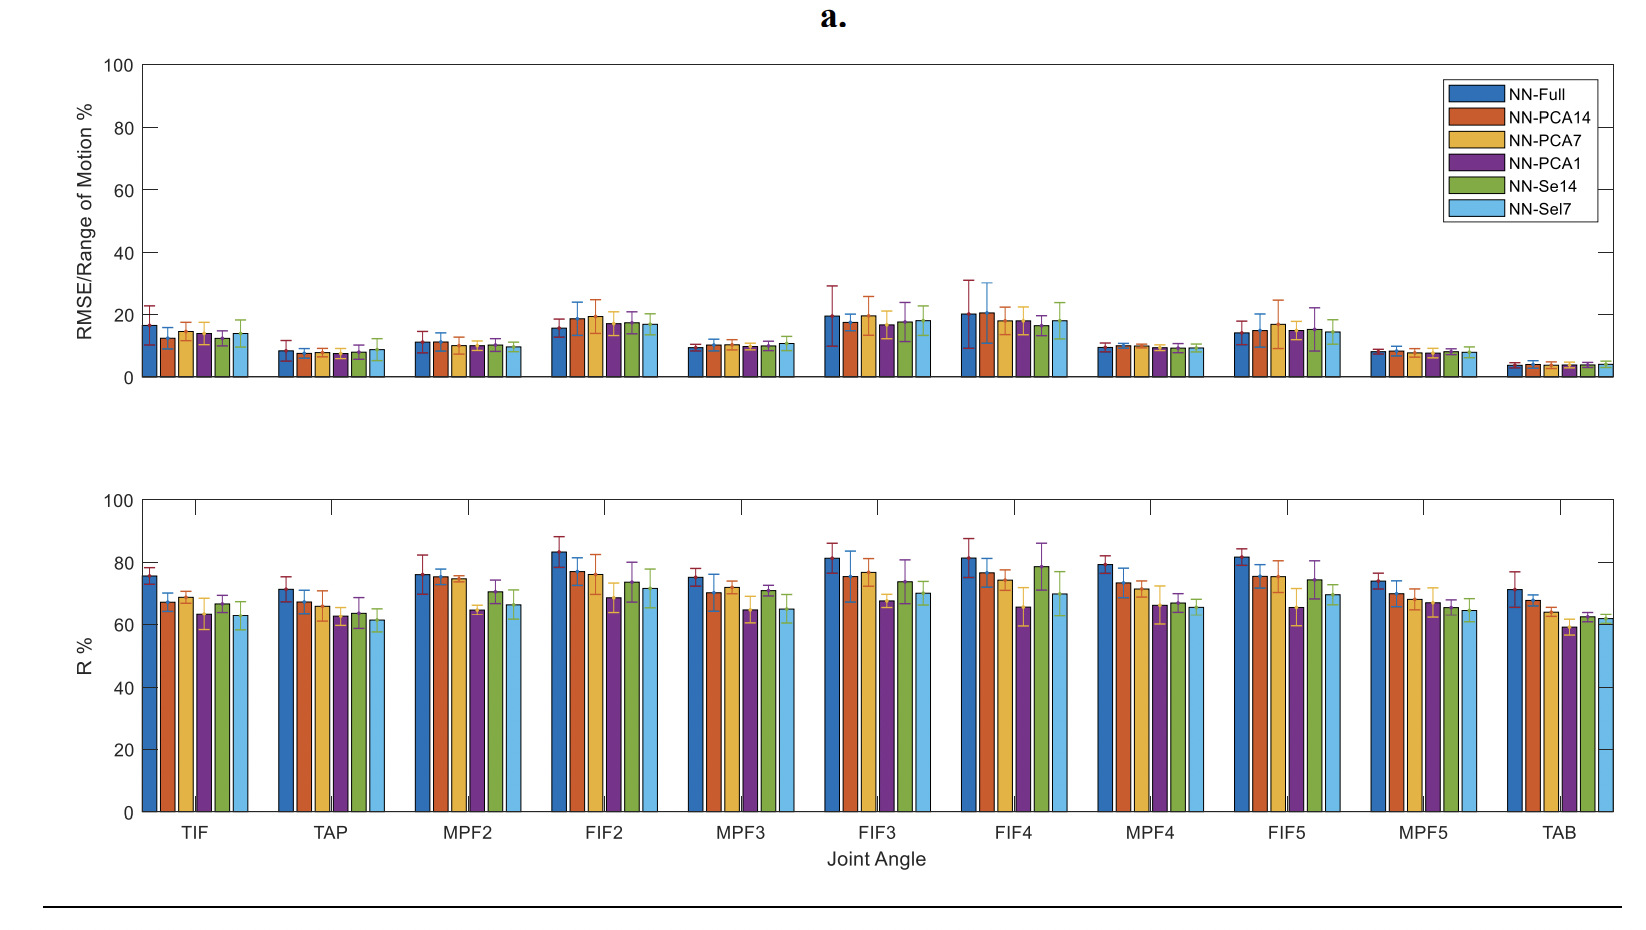
\includegraphics[width=\columnwidth]{figure7.png}
    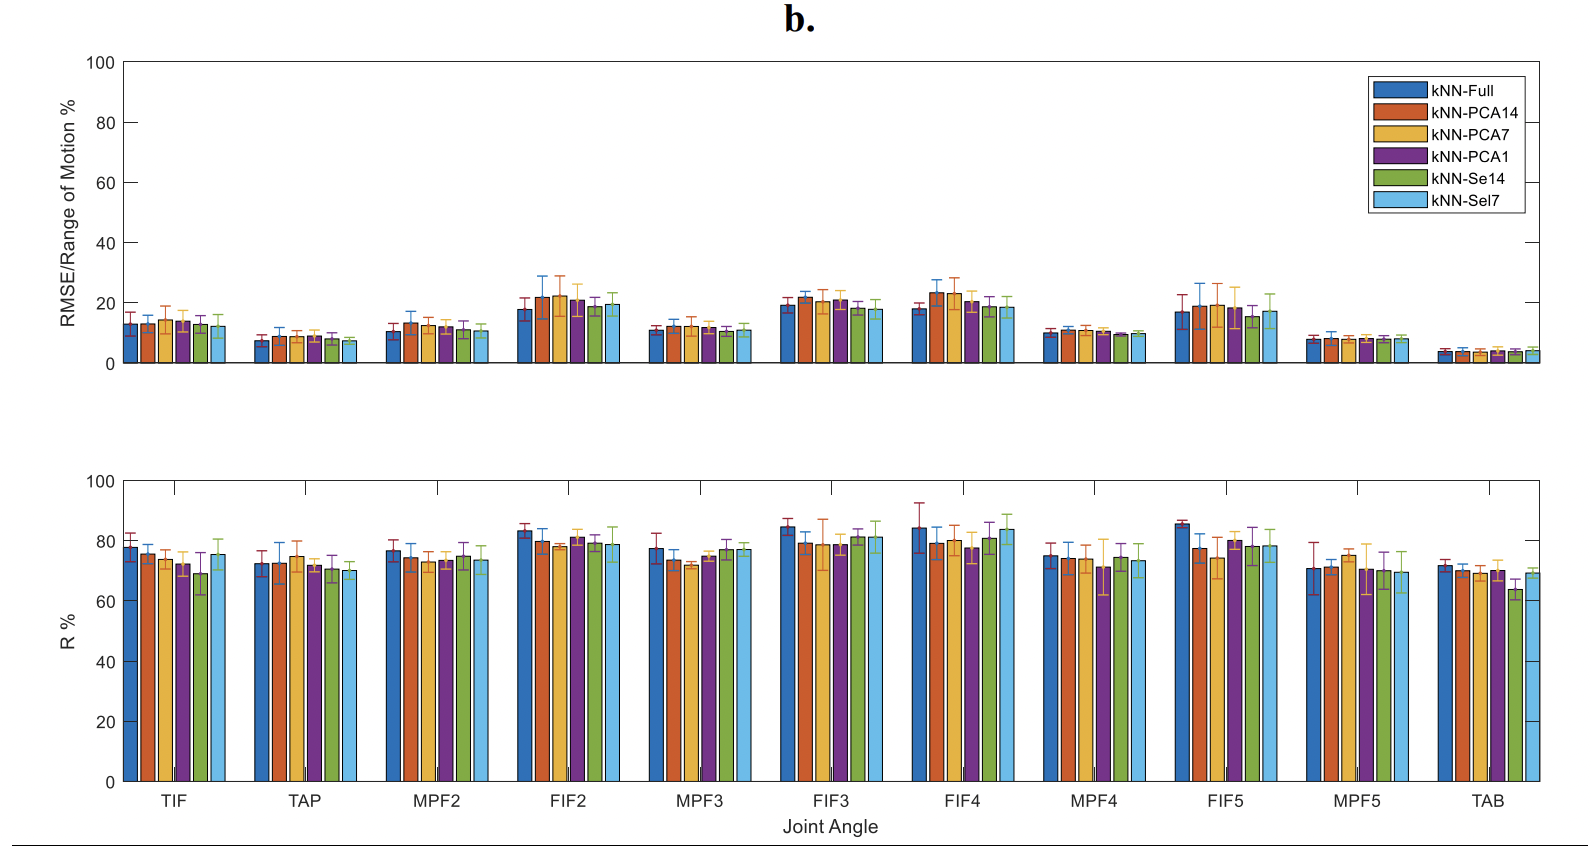
\includegraphics[width=\columnwidth]{figure8.png}
    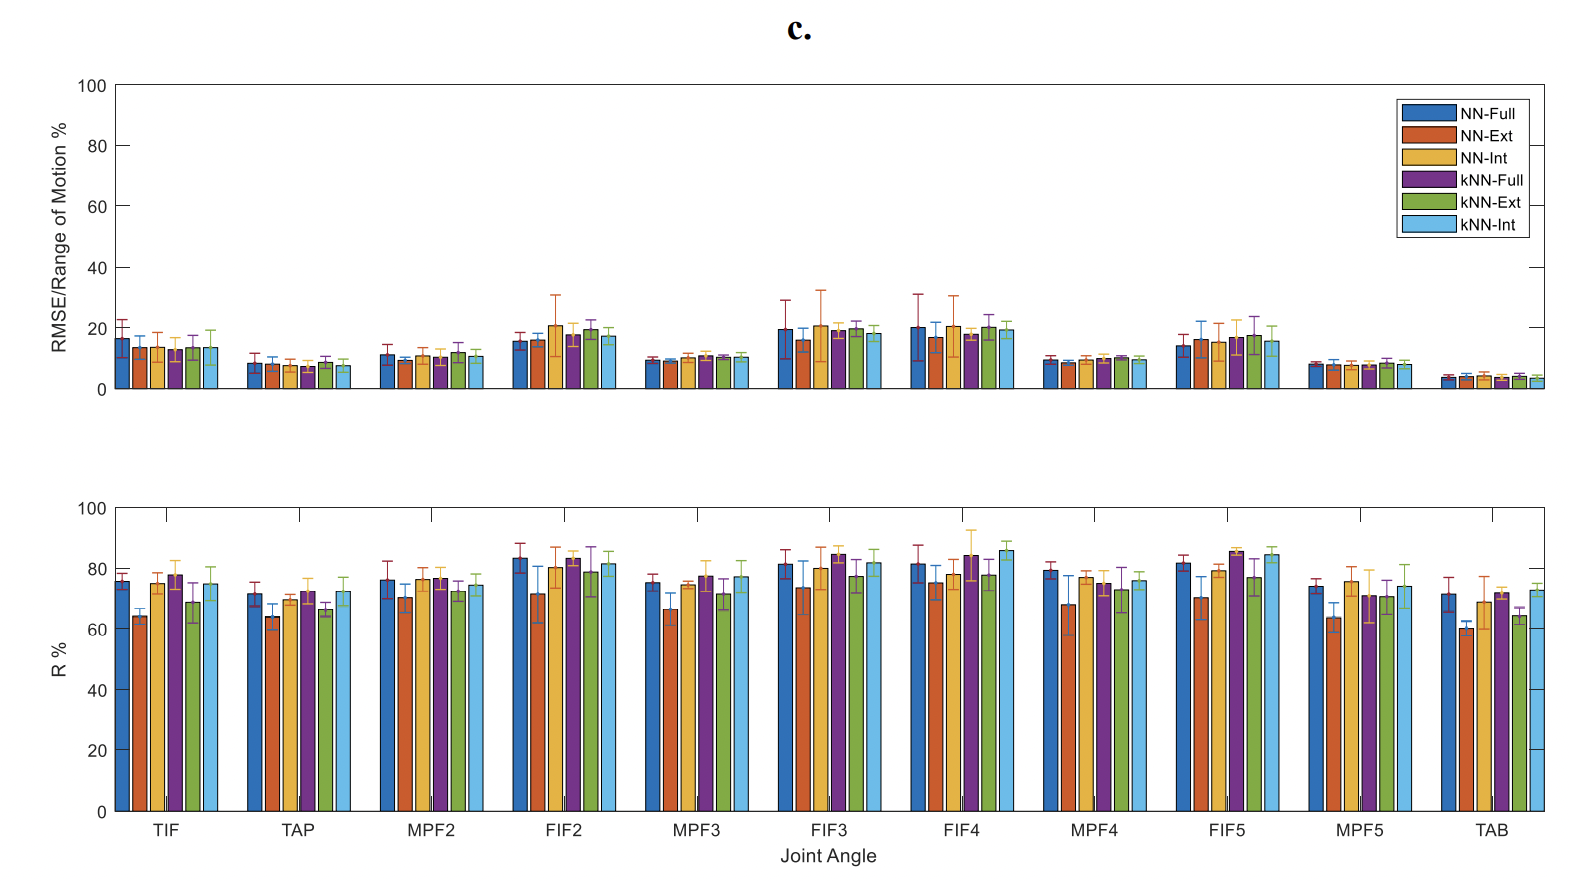
\includegraphics[width=\columnwidth]{figure9.png}
    \caption{RMSE (lower is better) and R-value (higher is better) in \textbf{a.)} NN and \textbf{b.)} kNN with different input features size. \textbf{c.)} RMSE and R-value in both NN and kNN, along with the use of only extrinsic/intrinsic muscles. The x-axis represents 
the joint angles, Full: using all bipolar channels, PCA14-7-1: using 14,7,1 first principal components, 
Sel14-7: using 14,7 selected channels, Ext: using only extrinsic grids, and Int: using only intrinsic grids.
}
    \label{figure7}
\end{figure}

\section{Discussion}
The proposed method in this study provides an alternative to estimate simultaneously eleven joint 
angles of the hand by using high-density surface EMG. The performance of the proposed method was 
comparable to previous similar studies \cite{b16}\cite{b19}\cite{b20}, albeit using more complex gestures to be estimated. 
The use of simple Neural Network and \textit{k}-Nearest Neighbour, however, gave this method a faster and lighter 
computation compared to the Gaussian Process proposed by Ngeo \textit{et al.} \cite{b16}. Although using time-domain 
features (RMS), the inclusion of intrinsic hand muscles in this study made an equivalent performance 
compared to the method proposed by Chen et al. \cite{b19}.

\subsection{Feature Dimensions}
As the result suggested, the use of 14 channels along the length of the HD-EMG grids (visually selected 
or generated by PCA) could give a reasonable estimation of the joints angle, comparable with the use the 
full grids. Although slightly reduced, the seven channels were also estimated the joint angle well (R=~70\% 
and RMSE=~11\%). The PCA, however, delivered a better estimation (not significantly), because the values 
in PCA were the projected values of all dimensions, contrary to the real reduced data in visually selected 
features \cite{b37}. Although the first principal component already explained ~70 \% of the data, the resulted 
estimation using this feature failed to produce an excellent performance (R=~65\% and RMSE=~19\%). 
Muceli and Farina \cite{b9} also reported that the more the channels used the better the performance of the 
regression. Although in that study, the full grids performed much better (significantly different, p$<<$0.001) 
than the reduced-channel configuration.
This explanation suggested that in the real implementation, the use of a long array of bipolar electrodes 
(placed perpendicularly against the vector of the muscle fibre) sufficed to control hand exoskeleton 
proportionally. This is also because, anatomically, the hand muscles are distributed in a radial manner \cite{b38}. 
Most of the commercialised product of myo-control also incorporated perpendicular electrode placements.
The inclusion of intrinsic muscles (full grids configuration) proved to give better performance, 
compared to the use of only extrinsic muscles (about 10\% better overall). This is because the extrinsic 
muscles are also consisted of other muscles to actuate the wrist, which will affect the EMG recording \cite{b39}.
As also suggested in section 3.B and \textbf{Figure 7c}, both the regressors (NN and kNN) combined with only 
intrinsic muscles as input features gave an equivalent performance with full grids configuration, and 
significantly better if compared with extrinsic only configuration. This implies that we can use only intrinsic 
muscles to predict the fingers kinematics \cite{b22}.
The dimension of the output feature (multiple DOFs of the hand) may as well be reduced because most 
of the time hand posture/gesture can be explained by its several components \cite{b32}\cite{b28}. Two principal 
components of the hand kinematics in this study sufficed to explain ~80 \% the data variance. As evident in 
\textbf{Figure 5b}, reducing the output into only two PCs might also help the practical aspect of regression in terms 
of alphabets recognition (not fully reported in this paper). This is based on the distinct distribution of 2 first 
PCs of alphabets gesture in \textbf{Figure 5b}. However, in \textbf{Figure 5b}, the O gesture could be falsely recognised as 
false-positive C. This is because the difference between O and C gestures are hardly distinguishable in terms 
of joints angle and muscle activity (\textbf{Figure 2}). Using three first PCs distribution proves to be 
harder in terms of recognition of the alphabets because the predicted kinematics did not fall to the area of 
target alphabets.

\subsection{Regression Method}
\textit{k}-Nearest Neighbour, interestingly, performed as good as, the more popularly used, Neural Network in 
regression. Although in reduced input feature configurations, kNN overall performed better than NN. This
is also proved by the comparable performance between full grids and reduced channels configurations in 
kNN (in NN, reducing the channels affected the performance). This difference is based on the technique used in both regressors. The NN is a data-driven method, meaning it will have a better chance at predicting 
values with more data given in the training phase \cite{b16}. The kNN is more pattern-driven method which means 
as long as the output value is one, it will recognise any pattern (input features) correctly \cite{b35}.

Compared to Gaussian Process proposed by Ngeo \textit{et al.} \cite{b16}, the kNN performed much faster with 
similar or comparable performance. The kNN was also able to predict more hand’s DOFs compared to the 
biomechanical model of Blana et al. \cite{b20}, with comparable processing time. In a practical aspect, kNN also 
performed significantly faster than NN (depends on the machine used). It will help later on real-time 
proportional control of hand exoskeleton because, in practical aspect, low computational time can reduce the 
lag between the user muscle activity and exoskeleton actuation \cite{b20}.

\subsection{Future and Implementation}
The process of joint angle estimation in this study was entirely done offline, but the proposed method 
is also feasible in online cases. It should be noted that the high dimensionality of the HD-EMG (using only 
RMS feature) can reduce the processing time by the use of simple regression method (NN and kNN) in 
contrast with more complex feature and regressor used in other studies \cite{b16}\cite{b19}. This implies that the delay 
in practical usage will be minimum ($<$~100 ms) to achieve real-time proportional control, although the 
increase of computational power in practical devices can enhance the processing time of sophisticated
methods. In the future, the use of a real or virtual exoskeleton hand should also be considered to check the 
proposed method practicality.
The subjects in this study were limited to a small number of healthy normal-bodied human. For the next 
development, a higher number of subjects and non-healthy volunteers should be considered for the result to 
be more established. The experiment of the study was also limited to a static arm and wrist position to reduce 
the possibility of wrist motion influence \cite{b39}. Fortunately, this problem can theoretically be solved by only 
incorporating intrinsic muscle as an input feature. To utilise the proposed strategy for estimating joint angle 
in clinical settings, a less complicated setup to measure the hand kinematics can be used, e.g. inertial 
measurement unit (IMU) sensor for each finger \cite{b40}.
Both HD-EMG and hand kinematics have redundant information on muscular-postural activities.
Analysis of postural and muscular synergy \cite{b36} can be applied to reduce the redundancy for more optimum 
and cost-effective usage although it can be very task-specific \cite{b41} if the muscle-posture activities involved 
in the study are not diverse enough.

\section{Conclusion}
The study in this paper has proposed a method to estimate eleven DOFs finger kinematics of 
sophisticated ASL gestures simultaneously by using HD-EMG from extrinsic and intrinsic muscles. The 
reduction of HD-EMG data did not affect the system's performance. Moreover, the intrinsic muscles were 
also superior compared to extrinsic muscles for estimating the hand kinematics. Furthermore, the kNN 
regressor performed better and faster compared to the NN, especially with the reduced input features. This 
proposed approach can also be utilised as a potentially practical solution for hand kinematics estimation in 
an exoskeleton.

\section*{Acknowledgement}
The author would like to thank Professor Dario Farina and Dr Silvia Muceli for the insight and general support to the study and Dr Alessandro Del Vecchio for discussion of the project plan.

All thanks also for the people of Neurorehabilitation Engineering Laboratory - Imperial College London, especially Karan Chugani and Simone Tanzarella for the technical support in the experiment.


\begin{thebibliography}{00}
%\bibitem{b1} S. B. Godfrey et al., “The Softhand Pro: Functional evaluation of a novel, flexible, and robust myoelectric prosthesis,” PLoS One, vol. 13, no. 10, pp. 1–20, 2018.

%\bibitem{b3} N. Jiang, J. L. Vest-Nielsen, S. Muceli, and D. Farina, “EMG-based simultaneous and proportional estimation of wrist/hand kinematics in uni-lateral trans-radial amputees,” J. Neuroeng. Rehabil., vol. 9, no. 1, 2012.
%\bibitem{b4} Ottobock, “bionic hand - Ottobock USA,” 2017. [Online]. Available: https://www.ottobockus.com/prosthetics/upper-limb-prosthetics/solution-overview/bebionic-hand.
%\bibitem{b5} “Open Bionics - turning disabilities into superpowers.” [Online]. Available: https://openbionics.com/.
%\bibitem{b6} M. B. I. Reaz, M. S. Hussain, and F. Mohd-Yasin, “Techniques of EMG signal analysis: detection, processing, classification and applications,” Biol. Proceed. Online, vol. 8, no. 1, pp. 11–35, 2006.
%\bibitem{b7} S. Negi, Y. Kumar, and V. M. Mishra, “Feature extraction and classification for EMG signals using linear discriminant analysis,” Proc. - 2016 Int. Conf. Adv. Comput. Commun. Autom. (Fall) ICACCA,2016, pp. 1–6, 2016.
%\bibitem{b8} O. Sandoval-Gonzalez et al., “Design and development of a hand exoskeleton robot for active and passive rehabilitation,” Int. J. Adv. Robot. Syst., vol. 13, no. 2, 2016.

%\bibitem{b10} R. F. Becker, “The cerebral cortex of man. By Wilder Penfield and Theodore Rasmussen. The Macmillan Company, New York, N.Y. 1950. 248 pp,” Am. J. Phys. Anthropol., vol. 11, no. 3, pp. 441–444, 1953.
\bibitem{b11} D. Leonardis et al., “An EMG-controlled robotic hand exoskeleton for bilateral rehabilitation,” IEEE Trans. Haptics, vol. 8, no. 2, pp. 140–151, 2015.
\bibitem{b12} Y. Yun et al., “Maestro: An EMG-driven assistive hand exoskeleton for spinal cord injury patients,” Proc. - IEEE Int. Conf. Robot. Autom., pp. 2904–2910, 2017.
\bibitem{b13} H. C. Siu, A. M. Arenas, T. Sun, and L. A. Stirling, “Implementation of a surface electromyography-based upper extremity exoskeleton controller using learning from demonstration,” Sensors 
(Switzerland), vol. 18, no. 2, pp. 0–20, 2018.
\bibitem{b14} R. J. Smith, F. Tenore, D. Huberdeau, R. Etienne-cummings, and N. V Thakor, “Continuous Decoding 
of Finger Position from Surface EMG Signals for the Control of Powered Prostheses,” Crit. Rev., pp. 
197–200, 2009.
\bibitem{b15} M. Hioki and H. Kawasaki, “Estimation of Finger Joint Angles from sEMG Using a Neural Network 
Including Time Delay Factor and Recurrent Structure,” ISRN Rehabil., vol. 2012, pp. 1–13, 2012.
\bibitem{b16} J. G. Ngeo, T. Tamei, and T. Shibata, “Continuous and simultaneous estimation of finger kinematics 
using inputs from an EMG-to-muscle activation model,” J. Neuroeng. Rehabil., vol. 11, no. 1, pp. 1–
14, 2014
\bibitem{b17} J. Ngeo, T. Tamei, and T. Shibata, “Estimation of continuous multi-DOF finger joint kinematics from surface EMG using a multi-output Gaussian Process,” 2014 36th Annu. Int. Conf. IEEE Eng. Med. Biol. Soc. EMBC, 2014, pp. 3537–3540, 2014.
\bibitem{b18} J. Ngeo et al., “Control of an optimal finger exoskeleton based on continuous joint angle estimation 
from EMG signals,” Proc. Annu. Int. Conf. IEEE Eng. Med. Biol. Soc. EMBS, pp. 338–341, 2013.
\bibitem{b19} C. Chen, G. Chai, W. Guo, X. Sheng, D. Farina, and X. Zhu, “Prediction of finger kinematics from 
discharge timings of motor units: Implications for intuitive control of myoelectric prostheses,” J. 
Neural Eng., vol. 16, no. 2, 2019.
\bibitem{b20} D. Blana, W. Murray, A. Ganguly, A. Krasoulis, K. Nazarpour, and E. Chadwick, “Model-based 
control of individual finger movements for prosthetic hand function,” Keele Univ., pp. 1–9, 2019.
\bibitem{b9} S. Muceli and D. Farina, “Simultaneous and proportional estimation of hand kinematics from EMG during mirrored movements at multiple degrees-of-freedom,” IEEE Trans. Neural Syst. Rehabil. Eng., vol. 20, no. 3, pp. 371–378, 2012.

\bibitem{b2} N. Celadon, S. Došen, I. Binder, P. Ariano, and D. Farina, “Proportional estimation of finger movements from high-density surface electromyography,” J. Neuroeng. Rehabil., vol. 13, no. 1, pp. 1–19, 2016.

\bibitem{b21} R. Merletti, A. Holobar, and D. Farina, “Analysis of motor units with high-density surface 
electromyography,” J. Electromyogr. Kinesiol., vol. 18, no. 6, pp. 879–890, 2008.
\bibitem{b22} A. A. Adewuyi, L. J. Hargrove, and T. A. Kuiken, “An Analysis of Intrinsic and Extrinsic Hand Muscle EMG for Improved Pattern Recognition Control.,” IEEE Trans. neural Syst. Rehabil. Eng. a Publ. IEEE Eng. Med. Biol. Soc., vol. 24, no. 4, pp. 485–494, Apr. 2016.
\bibitem{b23} M. Jordanic, M. Rojas-Martínez, M. A. Mañanas, and J. F. Alonso, “Spatial distribution of HD-EMG 
improves identification of task and force in patients with incomplete spinal cord injury,” J. Neuroeng. 
Rehabil., vol. 13, no. 1, pp. 1–11, 2016.
\bibitem{b24}  M. Barsotti, S. Dupan, I. Vujaklija, S. Dosen., A. Frisoli, and D. Farina, “Online finger control using high-density EMG and minimal training data for robotic applications,” IEEE Robot. Autom. Lett., vol. 4, no. 2, pp. 1–1, 2018.
\bibitem{b25} I. Carpinella, P. Mazzoleni, M. Rabuffetti, R. Thorsen, and M. Ferrarin, “Experimental protocol for 
the kinematic analysis of the hand: Definition and repeatability,” Gait Posture, vol. 23, no. 4, pp. 
445–454, 2006.
\bibitem{b26} “Hand drawn sign language alphabet Vector Free Download.” [Online]. Available: 
\textit{https://www.freepik.com/free$-$vector/hand$-$drawn$-$sign$-$language$-$ alphabet$_$1029740.html}}

\bibitem{b27} W. Geng, Y. Hu, Y. Wong, W. Wei, Y. Du, and M. Kankanhalli, “A novel attention-based hybrid CNN-RNN architecture for sEMG-based gesture recognition,” PLoS One, vol. 13, no. 10, pp. 1–18, 2018.
\bibitem{b28} E. J. Weiss and M. Flanders, “Muscular and postural synergies of the human hand,” J. Neurophysiol., vol. 92, no. 1, pp. 523–535, 2004.
\bibitem{b29} T. S. Buchanan, D. G. Lloyd, K. Manal, and T. F. Besier, “Comparison between different muscular 
models,” Neuromusculoskel. Model. Estim. Muscle Forces Jt. Moments Movements From Meas. 
Neural Command, vol. 20, no. 4, pp. 367–395, 2004.
\bibitem{b30} I. Vujaklija, V. Shalchyan, E. N. Kamavuako, N. Jiang, H. R. Marateb, and D. Farina, “Online 
mapping of EMG signals into kinematics by autoencoding,” J. Neuroeng. Rehabil., vol. 15, no. 1, pp. 
1–9, 2018.
\bibitem{b31} B. A. Kent, N. Karnati, and E. D. Engelberg, “Electromyogram synergy control of a dexterous 
artificial hand to unscrew and screw objects JNER JOURNAL OF NEUROENGINEERING AND 
REHABILITATION Electromyogram synergy control of a dexterous artificial hand to unscrew and
screw objects,” J. Neuroeng. Rehabil., vol. 11, p. 41, 2014
\bibitem{b32} M. Santello, M. Flanders, and J. F. Soechting, “Postural Hand Synergies for Tool Use,” J. Neurosci., 
vol. 18, no. 23, pp. 10105–10115, 1998.
\bibitem{b33} Y. Guo, S. Gok, and M. Sahin, “Convolutional networks outperform linear decoders in predicting 
EMG from spinal cord signals,” Front. Neurosci., vol. 12, no. OCT, 2018.
\bibitem{b34} T. Bao, A. Zaidi, S. Xie, and Z. Zhang, “Surface-EMG based Wrist Kinematics Estimation using 
Convolutional Neural Network,” pp. 1–4, 2019.
\bibitem{b35} T. Kumar, “Solution of linear and non-linear regression problem by K nearest neighbour approach: 
By using three-sigma rule,” Proc. - 2015 IEEE Int. Conf. Comput. Intell. Commun. Technol. CICT,
2015, pp. 197–201, 2015.
\bibitem{b36} M. Santello et al., “Hand synergies: Integration of robotics and neuroscience for understanding the 
control of biological and artificial hands Marco,” pp. 1–23, 2018.
\bibitem{b37} I. Jolliffe, “Principal component analysis. Springer Series in Statistics,” Encycl. Stat. Behav. Sci., p. 
487, 2002.
\bibitem{b38} M. Rojas-Martínez, M. A. Mañanas, and J. F. Alonso, “High-density surface EMG maps from upper-arm and forearm muscles,” J. Neuroeng. Rehabil., vol. 9, no. 1, pp. 1–17, 2012.
\bibitem{b39} N. Jiang, S. Muceli, B. Graimann, and D. Farina, “Effect of arm position on the prediction of 
kinematics from EMG in amputees,” Med. Biol. Eng. Comput., vol. 51, no. 1–2, pp. 143–151, 2013.
\bibitem{b40} B.-S. Lin, I.-J. Lee, P.-Y. Chiang, S.-Y. Huang and C.-W. Peng, “A Modular Data Glove System for 
Finger and Hand Motion Capture Based on Inertial Sensors,” J. Med. Biol. Eng., vol. 39, no. 4, pp. 
532–540, Aug. 2019.
\bibitem{b41} R. S. Razavian, N. Mehrabi, and J. McPhee, “A model-based approach to predict muscle synergies 
using optimization: Application to feedback control,” Front. Comput. Neurosci., vol. 9, no. OCT, pp. 
1–13, 2015.
\end{thebibliography}

\end{document}
